
\section{WDH: Turingmaschine}

\subsection*{}
\begin{frame}
  \frametitle{Definition der TM}

  \begin{block}{Ganz genau}
    Eine Turingmaschine $T = (Z, z_0, X, f, g, m)$ ist festgelegt durch
\begin{itemize}
	\item eine endlichen \textbf{Zustandsmenge} $Z$
	\item einen \textbf{Anfangszustand} $z_0 \in Z$
	\item ein endliches \textbf{Bandalphabet} $X$
	\pause
	\item eine partielle \textbf{Zustandsüberführung}sfunktion $f : Z \times X \dashrightarrow  Z$
	\item eine partielle \textbf{Ausgabe}funktion $g : Z \times X \dashrightarrow  X$ und
	\item eine partielle \textbf{Bewegung}sfunktion $m : Z \times X \dashrightarrow  \{-1, 0, 1\}$\end{itemize}
\end{block}
\end{frame}

\subsection*{}
\begin{frame}
  \frametitle{Definiton der TM}

  \begin{block}{Anmerkungen}
\begin{itemize}
	\item Die Funktionen \textbf{f}, \textbf{g} und \textbf{m} beschreiben zusammen, wie das aktuell eingelesene Zeichen verarbeitet werden soll (haben gemeinsamen Definitionsbereich).
	\pause
	\item Bei der Bewegungsfunktion bedeutet \textbf{-1 oder L} eine Bewegung des Lese-/Schreibkopfes nach links, \textbf{1 oder R}
eine Bewegung nach rechts und \textbf{0 oder N} ein Stehenbleiben.
\end{itemize}
\end{block}
\end{frame}

\subsection*{}
\begin{frame}
  \frametitle{Bekanntes Beispiel}
      \begin{center}
           \begin{tikzpicture}[shorten >=1pt,initial text=,node distance=1.5cm,auto,->,>=stealth,baseline=(B.base)]
             %\node[state,initial]  (S)                       {$S$};
             \node[state,initial]  (A)          {$A$};
             % \node (nix) [right of=A] {};
             \node[state]          (B) [above right of=A] {$B$};
             \node[state]          (C) [right of=B, node distance=2.5cm] {$C$};
             \node[state]          (E) [below right of=A] {$E$};
             \node[state]          (D) [right of=E, node distance=2.5cm] {$D$};


             \path[->]
             %(S) edge              node  {$$\square$\io$\square$R$} (A)
             (A) edge              node  {$1 | X R$} (B)
             (B) edge [loop above] node  {$1 | 1 R$} ()
             edge              node  {$\square | \square R$} (C)
             (C) edge [loop above] node  {$ 1 | 1 R$} ()
             edge              node  {$\square | 1 L$} (D)
             (D) edge [loop below] node  {$ 1 | 1 L$} ()
             edge              node  {$\square | \square L$} (E)
             (E) edge [loop below] node  {$ 1 | 1 L$} ()
             edge              node  {$ X | 1 R$} (A)
             % (B) edge              node        {$\square$\io$\square$R$} (B)
             % edge [loop right] node        {$1$\io$1$R$} ()
             % (B) edge [loop right] node {$\square$\io$1$L$} ()
             % edge  node [pos=0.3]       {$1$\io$1$L$} (A)
             ;
           \end{tikzpicture}
   				\begin{tabular}[t]{c|>{$}c<{$}@{\qquad}*{5}{c}}
            & A       & B      & C       & D       & E \\
            \hline
    		$\square$  &  & $\square$,R,C & 1,L,D & $\square$,L,E  &  \\
            1         & X,R,B & 1,R,B& 1,R,C & 1,L,D & 1,L,E \\
            X         &         &        &        &         & 1,R,A \\
          \end{tabular}
      \end{center}
\end{frame}

\subsection*{}
\begin{frame}
  \frametitle{Konfiguration einer TM}
Eine Turingmaschine befindet sich zu jedem Zeitpunkt in einem \textit{Gesamtzustand}, der als \textbf{Konfiguration} $(z, b, p) \in Z \times X^\mathbb{Z} \times \mathbb{Z}$ bezeichnet wird
\begin{block}{Vollständig beschrieben durch...}
\begin{itemize}
  \pause
	\item den aktuellen \textbf{Zustand} $z \in Z$ der Steuereinheit,
	\pause
	\item die aktuelle \textbf{Beschriftung des gesamten Bandes}, die man als Abbildung $b: \mathbb{Z} \rightarrow X$ formalisieren kann, und
	\pause
	\item die aktuelle \textbf{Position} $p \in Z$ \textbf{des Kopfes}.
\end{itemize}
\end{block}
\end{frame}

\subsection*{}
\begin{frame}
  \frametitle{Berechnungsschritt, d.h. Konfigurationswechsel}
  \pause
  Die \textbf{Menge aller Konfigurationen} bezeichnen wir als $\mathbb{C}_t$
  \pause
  \begin{block}{Schritt einer TM}
\begin{itemize}
	\item   $\Delta_x : \mathbb{C}_t \dashrightarrow  \mathbb{C}_t$
  \item		$\Delta_1(c)$ liefert direkte Nachfolgekonfiguration zu c
\end{itemize}
  \end{block}
  \pause
    \begin{block}{Endkonfigurationen einer TM}
  ist erreicht, falls $\Delta_1(c)$ nicht definiert ist
  \end{block}
\end{frame}

\subsection*{}
\begin{frame}
  \frametitle{Arten der Berechnung}

  \pause
  \begin{block}{endliche Berechnung}
\begin{itemize}
	\item endliche Folge von Konfigurationen $(c_0, c_1, c_2, . . . , c_t )$,
	\item wobei $0 < i \leq t$ gilt  $c_i = \Delta_1(c_{i-1})$
\end{itemize}
  \end{block}

  \pause
  \begin{block}{haltende Berechnung}
\begin{itemize}
	\item endliche Berechnung
	\item deren letzte Konfiguration eine Endkonfiguration ist
\end{itemize}
  \end{block}

  \pause
  \begin{block}{unendliche Berechnung}
\begin{itemize}
	\item unendliche Folge von Konfigurationen $(c_0, c_1, c_2, . . . )$
	\item wobei für $i>0$ gilt  $c_i = \Delta_1(c_{i-1})$
	\item \textbf{nicht haltend}
\end{itemize}
  \end{block}
\end{frame}

\subsection*{}
\begin{frame}
  \frametitle{Turingmaschinenakzeptoren}
  \pause
  \begin{block}{analog zu endlichen Automaten}
\begin{itemize}
	\item   \textbf{Erkennung formaler Sprachen}: ein Bit akzeptiert/abgelehnt
	\pause
  \item		Teilmenge $F \subset Z$ \textbf{akzeptierender Zustände}
  \item		TM akzeptiert Eingabewort $w$, wenn
\begin{itemize}
	\pause
	\item TM für Eingabe $w$ hält und
	\pause
	\item der Zustand der Endkonfiguration $\Delta_{*}(c_0(w))$ akzepierend ist
\end{itemize}
\pause
\item $L(T)$: Menge der akzeptierten Wörter
\end{itemize}
\end{block}
\end{frame}

\subsection*{}
\begin{frame}
  \frametitle{Ihr seid dran...}
	\only<1>{
  \begin{block}{Aufgabe}
	Gebt ein TM-Akzeptor an, der die Sprache $L^= = \{0^n1^n : n \geq 1\}$ akzeptiert
	\end{block}}
  \only<2->{
\begin{block}{Lösung (die Markierung des Startzustands fehlt)}
\begin{figure}
	\centering
		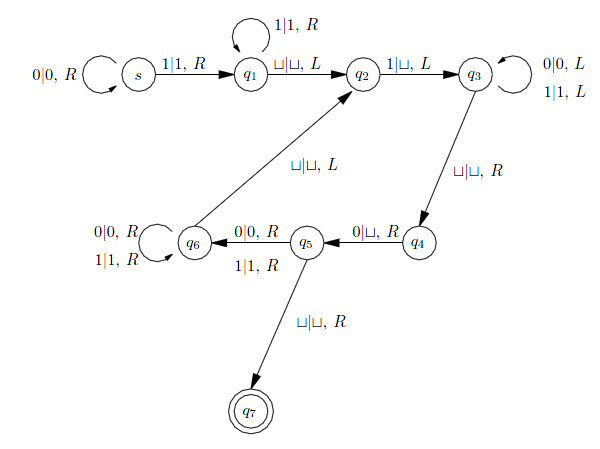
\includegraphics[height=6.7cm]{src/tut13_tmaufgabe.png}
\end{figure}
\end{block}}
\end{frame}

\subsection*{}
\begin{frame}
  \frametitle{Aufzählbare und entscheidbare Sprachen}
  \begin{block}{zwei Möglichkeiten, wenn $w$ von TM nicht akzeptiert wird}
\begin{enumerate}
\pause
	\item TM hält für Eingabe $w$, aber Endzustand nicht akzeptierend
	\pause
  \item	TM hält für Eingabe $w$ \textbf{nicht}
\end{enumerate}
\end{block}
\pause
  \begin{block}{Was wissen wir über die Berechnung?}
\begin{enumerate}
\pause
	\item TM ist fertig und lehnt die Eingabe ab
\pause
  \item	TM ist noch nicht fertig (\textit{Ob TM irgendwann w noch akzeptiert oder ablehnt, ist unklar!})
\end{enumerate}
\end{block}
\pause
  \begin{block}{Wir halten in zwei Definitionen fest}
\begin{enumerate}
	\item $L$ heißt \textbf{entscheidbare Sprache}, wenn es eine TM gibt, die \textbf{immer hält} und $L$ akzeptiert.
	\pause
	\item $L$ heißt \textbf{aufzählbare}(semi-entscheidbar) \textbf{Sprache}, wenn es eine TM gibt, die $L$ akzeptiert
\end{enumerate}
\end{block}
\end{frame}

%%%%%%%%%%%%%%%%%%%%%%%%%%%%%% Unentscheidbare Probleme %%%%%%%%%%%%%%%%%%%%
\section{Unentscheidbare Probleme}

\subsection*{}
\begin{frame}
  \frametitle{Codierungen von Turingmaschinen}

  \begin{block}{Gödelisierung}
\begin{itemize}
\pause
	\item Ziel: Beschreibe jede Turingmaschine durch ein Wort
	\pause
	\item Verfahren: \textbf{Durch-Nummerierung} von Turingmaschinen
\begin{itemize}
  \item Triviales Alphabet zur Codierung wie z.B. $A = \{[, ], 0, 1\}$
\pause
	\item Codierung der Zustände, Symbole, Kopfbewegungen, Funktionen
	\pause
	\item Codierung der gesamten Turingmaschine als Konkatentation aller codierten Bestandteile
\end{itemize}
\end{itemize}
   \end{block}
\end{frame}

\subsection*{}
\begin{frame}
  \frametitle{Eigenschaften dieser Codierungen}

  \begin{block}{einfache Syntaxanalyse ist möglich}
\begin{itemize}
	\item TM konstruierbar, die für $w \in A^*$ feststellt, ob es die Codierung einer TM ist oder nicht.
\end{itemize}
  \end{block}
  \pause
  \begin{block}{\textbf{universelle Turingmaschine} $U$ existiert}
\begin{itemize}
\pause
	\item erhält als Eingabe zwei Argumente als Wort $[w_1][w_2]$
	\pause
	\item prüft, ob $w_1$ Codierung einer Turingmaschine $T$ ist
	\pause
	\item falls nein: hält mit NEIN
	\pause
	\item falls ja:
	\pause
\begin{itemize}
	\item U \textbf{simuliert Schritt für Schritt die Arbeit}, die $T$ für die Eingabe $w_2$ durchführen würde
	\pause
	\item $U$ liefert am Ende als Ergebnis, was $T$ liefern würde (\textit{FALLS T hält!})
\end{itemize}
\end{itemize}
  \end{block}
\end{frame}


\subsection*{}
\begin{frame}
  \frametitle{Das Halteproblem}

  \begin{block}{Das Halteproblem ist die formale Sprache}
  $H = \{w \in A^* | $w ist eine TM-Codierung und $T_w(w)$ hält. $\}$
   \end{block}
   \pause
   \begin{block}{Satz}
  Das \textbf{Halteproblem ist unentscheidbar}, d. h. es gibt keine TM, die das Problem entscheidet.
   \end{block}
   \pause
   \begin{block}{Anmerkung}
  \textbf{Aber:} Das Halteproblem ist aufzählbar(semi-entscheidbar). Man zeigt das mittels Univeral-TM.
   \end{block}
\end{frame}


%%%%%%%%%%%%%%%%%%%%%%%%%%%%%% Äquivalenzrelationen %%%%%%%%%%%%%%%%%%%%
\section[Relationen]{Äquivalenzrelationen}

\subsection*{}
\begin{frame}
  \frametitle{Definition von Äquivalenzrelationen}

	\begin{block}{Vorraussetzungen}
		\begin{description}
			\item[reflexiv] $x R x$
			\item[transitiv] Aus $x R y$ und $y R z$ folgt $x R z$
			\item[symmetrisch] Aus $x R y$ folgt $y R x$
		\end{description} \pause
		Gelten alle diese Eigenschaften für alle $x,y$, handelt es sich um eine \textbf{Äquivalenzrelation}.
	\end{block}
\end{frame}


\begin{frame}
  \frametitle{Äquivalenzrelationen}

  \begin{block}{Relation als Graph}
    \begin{itemize}
    \item Darstellung von Relationen als gerichtete Graphen:
      Woran sieht man
      \begin{itemize}
        \item Reflexivität?
        \item Symmetrie?
        \item Transitivität?
      \end{itemize} \pause
    \item Wie sieht der Graph einer Äquivalenzrelation aus: \pause
      "`Cliquen"', in denen jeder mit jedem verbunden ist
      \item dazwischen nichts (die Cliquen heißen später Äquivalenzklassen)
    \end{itemize}
   \end{block}
\end{frame}


\begin{frame}
  \frametitle{Äquivalenzrelationen von Nerode}

  \begin{block}{Definition}
  	für alle $w_1,w_2 \in A^*$ ist\\
  	$w1 \equiv_L w2 \Leftrightarrow (\forall w \in A^*: w_1w \in L \Leftrightarrow w_2w \in L)$

  	\pause
    \begin{itemize}
    \item das liest man besser mehrmals durch
    	\pause
      \begin{itemize}
      \item man nehme eine Sprache $L$, die von einem endlichen Akzeptor
        erkannt wird
      \item man nehme zwei Wörter $w_1$, $w_2$ die \emph{nicht}
        $\equiv_L$-äquivalent sind
      \item Was kann man über $f^*(z_0,w_1)$ und $f^*(z_0,w_2)$ sagen?\pause
      \item Sie müssen verschieden sein, denn sonst
        $f^*(z_0,w_1)=f^*(z_0,w_2)$ und dann auch für jedes Suffix
        $w$: $f^*(z_0,w_1w)=f^*(z_0,w_2w)$, also werden für jedes
        Suffix entweder beide Wörter $w_1w$ und $w_2w$ oder keines
        akzeptiert, und dann wären $w_1$ und $w_2$ ja äquivalent.
      \end{itemize}
    \end{itemize}

   \end{block}
\end{frame}


\begin{frame}
  \frametitle{Äquivalenzrelationen von Nerode}

  \begin{block}{Beispiele}
	aus dem Skript:\\
	Sei $L = \langle a*b* \rangle \subset A^*$
    \begin{itemize}
    	\item $w_1 = aaa, w_2 = a$
    	\item $w_1 = aaab, w_2 = abb$
    	\item $w_1 = aa, w_2 = abb$ \only<2>{ nicht $\equiv_L$-äquivalent sind}
    	\item $w_1 = aba, w_2 = babb$
    	\item $w_1 = ab, w_2 = ba$ \only<2>{ nicht $\equiv_L$-äquivalent sind}
    \end{itemize}

   \end{block}
\end{frame}

\section[Halbordnungen]{Halbordnungen}

\subsection*{}
\begin{frame}
  \frametitle{WDH: Definition von Äquivalenzrelationen}

	\begin{block}{Vorraussetzungen} \pause
		\begin{description}
			\item[reflexiv] $x R x$
			\item[transitiv] Aus $x R y$ und $y R z$ folgt $x R z$
			\item[symmetrisch] Aus $x R y$ folgt $y R x$
		\end{description} \pause
		Gelten alle diese Eigenschaften für alle $x,y,z \in M$, handelt es sich um eine \textbf{Äquivalenzrelation}.
	\end{block}
\end{frame}

\subsection*{}
\begin{frame}
  \frametitle{Definition einer Halbordnung}

	\begin{block}{Vorraussetzungen}
		\begin{description}
			\item[reflexiv] $x R x$
			\item[transitiv] Aus $x R y$ und $y R z$ folgt $x R z$ \pause
			\item[antisymmetrisch] Aus $x R y$ und $y R x$ folgt $x = y$
		\end{description} \pause
\begin{itemize}
	\item Gelten alle diese Eigenschaften für alle $x,y$, handelt es sich bei $R \subseteq M x M$ um eine \textbf{Halbordnung}. \pause
	\item	Wenn R Halbordnung auf Menge M ist, nennt man M eine \textbf{halbgeordnete Menge}.
\end{itemize}
	\end{block}
\end{frame}


\subsection*{}
\begin{frame}
  \frametitle{Beispiel Mengeninklusion}

	\begin{block}{Untersuchung der Mengeninklusion}
      Handelt es sich bei der Relation $\subseteq$ (Mengeninklusion) um eine \textbf{Äquivalenzrelation oder Halbordnung} auf Potenzmenge $P = 2^M$? \pause
\begin{itemize}
	\item relfexiv: $\forall A \in P$: $A \subseteq A$ \pause
	\item transitiv: $\forall A, B, C \in P$: $A \subseteq B$ und $B \subseteq C \Longrightarrow A \subseteq C$ \pause
	\item symmetrisch: $\forall A, B \in P$: $A \subseteq B \Longrightarrow B \subseteq A$
	\only<5->{ gilt nicht. \textbf{ABER:} Aus \textbf{keiner Symmetrie} folgt nicht notwendig die Antisymmetrie!
	}
	\only<6->{
	\item antisymmetrisch: $\forall A, B \in P$: $A \subseteq B$ und $B \subseteq A \Longrightarrow A = B$ (Analogie zur Mengengleichheit)
	}
\end{itemize}
	\only<7->{
	\textbf{Die Mengeninklusion ist eine Halbordnung.}
	}
  \end{block}
\end{frame}

\subsection*{}
\begin{frame}
  \frametitle{Ihr seid dran...}

	\begin{block}{Aufgabe}
	Überprüft, ob es sich bei folgenden Relationen um Halbordnungen handelt:
  \begin{itemize}
    \item  $\sqsubseteq_p$ auf $A^*$ mit $v\sqsubseteq_p w \Leftrightarrow \exists u: vu=w$ ?
      \only<2->{
      \begin{itemize}
      \item \textbf{Reflexivität}: gilt wegen  $w_1\epsilon=w_1$
      \item \textbf{Antisymmetrie}: wenn $w_1\sqsubseteq_p w_2$ und $w_2\sqsubseteq w_1$,
        dann gibt es $u_1,u_2\in A^*$ mit $w_1u_1=w_2$ und
        $w_2u_2=w_1$. Also ist $w_1u_1u_2=w_2u_2=w_1$. Also muss
        $|u_1u_2|=0$ sein, also $u_1=u_2=\epsilon$, also $w_1=w_2$.
      \item \textbf{Transitivität}: wenn $w_1\sqsubseteq_p w_2$ und $w_2\sqsubseteq w_3$,
        dann gibt es $u_1,u_2\in A^*$ mit $w_1u_1=w_2$ und
        $w_2u_2=w_3$.  Also ist $w_1(u_1u_2)=(w_1u_1)u_2=w_2u_2=w_3$,
        also $w_1\sqsubseteq w_3$.
      \end{itemize}
      }
   \only<3->{ \item $\sqsubseteq$ auf $A^*$ mit $w_1\sqsubseteq w_2 \Leftrightarrow |w_1| \leq |w_2|$ ? }
    \only<4->{
			\begin{itemize}
				\item Antisymmetrie ist verletzt.
				 \only<5->{ \item Reflexivität und Transitivität sind erfüllt. }
			\end{itemize}
		}
   \end{itemize}

  \end{block}
\end{frame}

\subsection*{}
\begin{frame}
  \frametitle{Hassediagramm}
  \begin{block}{Konstruktion}
  Zur \textbf{Veranschaulichung einer Halbordnung} lassen sich Hassediagramme folgendermaßen erstellen: \pause
    \begin{enumerate}
    \item Darstellung der Halbordnung als Graph \pause
    \item Entfernen aller reflexiven und transitiven Kanten
    \end{enumerate}
    	\end{block}
\end{frame}

\subsection*{}
\begin{frame}
  \frametitle{Extreme "`Elemente"' I}
  Sei $( M, \sqsubseteq )$ halbgeordnet und $T \subseteq M$ \pause
  \begin{block}{minimale und maximale Elemente}
    \begin{itemize}
    \item $x \in T$ heißt \textbf{minimales Element} von T, wenn es kein $y \in T$ gibt mit $y \sqsubseteq x$ und $y \neq x$. \pause
    \item $x \in T$ heißt \textbf{maximales Element} von T, wenn es kein $y \in T$ gibt mit $x \sqsubseteq y$ und $x \neq y$. \pause
    \end{itemize}
	\end{block}
	\begin{block}{kleinstes und größtes Element}
    \begin{itemize}
    \item $x \in T$ heißt \textbf{kleinstes Element} von T, wenn für alle $y \in T$ gilt: $x \sqsubseteq y$. \pause
    \item $x \in T$ heißt \textbf{größtes Element} von T, wenn für alle $y \in T$ gilt: $y \sqsubseteq x$.
    \end{itemize}
  \end{block}
  \only<6->{
  Eine Teilmenge T kann mehrere minimale (bzw. maximale) Elemente besitzen, aber nur ein kleinstes (bzw. größtes)!
  }
\end{frame}

\subsection*{}
\begin{frame}
  \frametitle{Beispiel mit Hassediagramm}
  \begin{block}{Beispiel}
    \begin{itemize}
    \item Male das Hassediagramm zur Halbordnung $(\{ \{\}, a, b, c, ab, bc, ac\}, \subseteq)$ \pause
    \item woran erkennt man Minima? \pause
    \item woran Maxima?
    \end{itemize}
	\end{block}
\end{frame}

\subsection*{}
\begin{frame}
  \frametitle{Extreme "`Elemente"' II}
  Sei $( M, \sqsubseteq )$ halbgeordnet und $T \subseteq M$ \pause
  \begin{block}{Untere und obere Schranken}
    \begin{itemize}
    \item $x \in M$ heißt \textbf{untere Schranke} von T, wenn für alle $y \in T$ gilt: $x \sqsubseteq y$. \pause
    \item $x \in M$ heißt \textbf{obere Schranke} von T, wenn für alle $y \in T$ gilt: $y \sqsubseteq x$.  \pause
    \end{itemize}
    \only<4->{
    Also: Schranken von T dürfen außerhalb von T liegen.
    }
	\end{block}
\end{frame}

\subsection*{}
\begin{frame}
  \frametitle{Extreme "`Elemente"' III}
	\begin{block}{Supremum und Infimum}
    \begin{itemize}
    \item Besitzt die Menge aller oberen Schranken einer Teilmenge T ein kleinstes Element, so heißt dies das \textbf{Supremum} von T ($sup(T)$) \pause
    \item Besitzt die Menge aller unteren Schranken einer Teilmenge T ein größtes Element, so heißt dies das \textbf{Infimum} von T ($inf(T)$) \pause
    \item \textbf{Achtung}: Existieren nicht, wenn
			\begin{itemize}
				\item überhaupt keine oberen (unteren) Schranken vorhanden \pause
				\item keine eindeutig kleinste (größte) Schranke aller oberer (unterer) Schranken
			\end{itemize}
		\end{itemize}
  \end{block}
\end{frame}

\subsection*{}
\begin{frame}
  \frametitle{Vollständige Halbordnungen}
  \begin{block}{aufsteigende Kette}
  wird definiert als
    \begin{itemize}
    \item abzählbar unendliche Folge $(x_0, x_1, x_2, ... )$ von Elementen
    \item mit Eigenschaft: $\forall i \in N_0$: $x_i \sqsubseteq x_{i+1}$
    \end{itemize}
	\end{block}
	\pause
	\begin{block}{vollständige Halbordnung}
    Eine Halbordnung heißt \textbf{vollständig}, wenn
    \begin{itemize}
    \item sie ein kleinstes Element $\bot$ hat und
    \item jede aufsteigende Kette $ x_0 \sqsubseteq x_1 \sqsubseteq x_2 \sqsubseteq ...$ ein Supremum $x_i$ besitzt
    \end{itemize}
	\end{block}
\end{frame}

\subsection*{}
\begin{frame}
  \frametitle{Vollständige Halbordnungen II}
  \begin{block}{Stetige Abbildungen auf vollständigen Halbordnungen}
    \begin{itemize}
    \item Beispiel aus dem Skript
    \item Gegeben sei:
    \item Terminalzeichenalphabet $T=\{a,b\}$, \pause
    \item $D$ die halbgeordnete Potenzmenge $D=2^{T^*}$ der Menge aller Wörter
    \item mit Inklusion als Halbordnungsrelation. \pause
    \item Elemente der Halbordnung sind also Mengen von Wörtern, d.h. formale Sprachen. \pause
    \item Kleinstes Element der Halbordnung ist die leere Menge $\emptyset$.  \pause
    \item Wie weiter vorne erwähnt, ist diese Halbordnung vollständig.
    \end{itemize}
	\end{block}
\end{frame}
\subsection*{}
\begin{frame}
  \frametitle{Vollständige Halbordnungen III}
  \begin{block}{Beweis}
    \begin{itemize}
    \item Es sei $v\in T^*$ ein Wort und $f_v:D\rightarrow D$ die Abbildung
      $f_v(L)=\{v\}L$, die vor jedes Wort von $L$ vorne $v$
      konkateniert.
    \item Behauptung: $f_v$ ist stetig.
    \item Beweis: Es sei $L_0\subseteq L_1\subseteq L_2\subseteq
      \cdots$ eine Kette und $L=\bigcup L_i$ ihr Supremum.

      $f_v(L_i)=\{ vw | w\in L_i \}$, also $\bigcup_i f_v(L_i)= \{ vw | \exists i\in N_0: w\in L_i\} = \{v\}\{w | \exists i \in N_0: w\in L_i\}$ $=\{v\}\bigcup_i L_i = f(\bigcup_i L_i)$.
    \item analog für Konkatenation von rechts
    \end{itemize}
	\end{block}
\end{frame}

\section[Ordnungen]{Ordnungen}
\subsection*{}
\begin{frame}
  \frametitle{Totale Ordnung}

	\begin{block}{Definition}
	Relation $R \subseteq M x M$ ist eine Ordnung oder genauer \textbf{totale Ordnung}, wenn
\begin{itemize}
	\item R Halbordnung ist \pause
	\item und gilt: $\forall x ,y \in M$: $x R y \vee y R x$
\end{itemize}
	\end{block}
\pause
	\begin{block}{Anmerkungen}
\begin{itemize}
	\item $\Rightarrow$ : Es gibt keine unvergleichbaren Elemente.
\end{itemize}
	\end{block}
\end{frame}

\subsection*{}
\begin{frame}
  \frametitle{Totale Ordnung}

	\begin{block}{Beispiele}
\begin{itemize}
	\item $( N_0 , \leq )$ \pause
	\item $( \{a, b\}^*, \sqsubseteq_1 )$ mit $w_1 \sqsubseteq_1 w_2$ "`wie im Wörterbuch"' \pause
	\item $( \{a, b\}^*, \sqsubseteq_2 )$ mit $w_1 \sqsubseteq_2 w_2$ genau dann, wenn \pause
		\begin{itemize}
			\item entweder $|w_1| < |w_2|$ \pause
			\item oder $|w_1| = |w_2|$ und $w_1 \sqsubseteq_1 w_2$ gilt
		\end{itemize}
\end{itemize}
	\end{block}
\end{frame}

\subsection*{}
\begin{frame}
  \frametitle{Ihr seid dran...}

	\begin{block}{Beispiele für $\sqsubseteq_1$:}
      \begin{itemize}
        \item  Warum ist $aa \sqsubseteq_1 aabba$? \pause
        \item  Warum ist $aa \sqsubseteq_1 bba$? \pause
        \item  Warum ist $aaaaa \sqsubseteq_1 bba$? \pause
        \item  Warum ist $aaaab \sqsubseteq_1 aab$? \pause
      \end{itemize}
  \end{block}
  \begin{block}{Beispiele für $\sqsubseteq_2$:}
      \begin{itemize}
        \item  Warum ist $aa \sqsubseteq_2 aabba$? \pause
        \item  Warum ist $aa \sqsubseteq_2 bba$? \pause
        \item  Warum ist $bba \sqsubseteq_2 aaaaa$? (vergleiche $\sqsubseteq_1$!)\pause
        \item  Warum ist $aab \sqsubseteq_2 aaaab$? (vergleiche $\sqsubseteq_1$!)
      \end{itemize}
	\end{block}
\end{frame}

\subsection*{}
\begin{frame}
  \frametitle{Bleibt dran...}

	\begin{block}{Aufgabe}
		Relation $\sqsubseteq_p$ auf $ \{a, b\}^* $ eine totale Ordnung?
	\end{block}
	\only<2->{
	\begin{block}{Lösung}
		Es handelt sich um eine Halbordnung, allerdings mit unvergleichbaren Element wie z.B. $a, b$.
		Daher ist die Relation $\sqsubseteq_p$ \textbf{keine} totale Ordnung.
	\end{block}
	}
\end{frame}


\section{Abschluss}
% Studis anzuregen darüber nachzudenken, ob sie wirklich alles wissen, ansonsten nachlesen oder fragen nachträglich stellen, dann kann in der nächsten Woche nochmal drauf eingegangen werden
\subsection*{}
\begin{frame}
	\frametitle{Zum Schluss...}
	\begin{block}{Was ihr nun wissen solltet!}
	\begin{itemize}
	  	\visible<2->{\item Was ist ein Algorithmus?}
		\visible<3->{\item Welche Arten von Berechnung unterscheiden wir?}
		\visible<4->{\item Was zeichnet das Halteproblem aus? Gibt es noch andere Probleme, auf die dasselbe zutrifft?}
		\visible<5->{\item Was besagt die Äquivalenzrelation von Nerode?}
    \end{itemize}
   	\end{block}

	\visible<6->{
	\begin{block}{Ihr wisst was nicht?}
		Stellt \textbf{jetzt} Fragen!
	\end{block}}
\end{frame}